%%%%%%%%%%%%%%%%%%%%%%% file template.tex %%%%%%%%%%%%%%%%%%%%%%%%%
%
% This is a general template file for the LaTeX package SVJour3
% for Springer journals.          Springer Heidelberg 2010/09/16
%
% Copy it to a new file with a new name and use it as the basis
% for your article. Delete % signs as needed.
%
% This template includes a few options for different layouts and
% content for various journals. Please consult a previous issue of
% your journal as needed.
%
%%%%%%%%%%%%%%%%%%%%%%%%%%%%%%%%%%%%%%%%%%%%%%%%%%%%%%%%%%%%%%%%%%%

%
\RequirePackage{fix-cm}
%
%\documentclass{svjour3}                     % onecolumn (standard format)
%\documentclass[smallcondensed]{svjour3}     % onecolumn (ditto)
\documentclass[smallextended]{svjour3}       % onecolumn (second format)
%\documentclass[twocolumn]{svjour3}          % twocolumn
%
\smartqed  % flush right qed marks, e.g. at end of proof
%
\usepackage{graphicx}
\usepackage{natbib}
%
% \usepackage{mathptmx}      % use Times fonts if available on your TeX system
%
% insert here the call for the packages your document requires
%\usepackage{latexsym}
% etc.
%
% please place your own definitions here and don't use \def but
% \newcommand{}{}
%
% Insert the name of "your journal" with
\journalname{Attention, Perception, \& Psychophysics}
%
\begin{document}

\title{Replicating the visual search visualisation experiment\thanks{Say thanks to Amelia's grant}}
\subtitle{Do the results stand up? Do they generalise?}

\titlerunning{Short form of title}        % if too long for running head

\author{Alasdair D. F. Clarke         \and
        Amelia R. Hunt
}

%\authorrunning{Short form of author list} % if too long for running head

\institute{F. Author \at
              first address \\
              Tel.: +123-45-678910\\
              Fax: +123-45-678910\\
              \email{fauthor@example.com}           %  \\
%             \emph{Present address:} of F. Author  %  if needed
           \and
           S. Author \at
              second address
}

\date{Received: date / Accepted: date}
% The correct dates will be entered by the editor


\maketitle

\begin{abstract}
Insert your abstract here. Include keywords, PACS and mathematical
subject classification numbers as needed.
\keywords{mental imagery \and visual attention, \and learning \and visual search \and perception \and open materials}
% \PACS{PACS code1 \and PACS code2 \and more}
% \subclass{MSC code1 \and MSC code2 \and more}
\end{abstract}

%%%%%%%%%%%%%%%%%%%%%%%%%%%%%%%%%%%%%%%%%%%%%%%%%%%%%
\section{Introduction}
\label{sec:intro}
%%%%%%%%%%%%%%%%%%%%%%%%%%%%%%%%%%%%%%%%%%%%%%%%%%%%%

Mental imagery, also referred to as visualising, is the phenomenon where by 
We are going to replicate \cite{reinhart2015}. We will also test if the study generalises. 

%%%%%%%%%%%%%%%%%%%%%%%%%%%%%%%%%%%%%%%%%%%%%%%%%%%%%
\section{Experiment 1}
\label{sec:exp1}
%%%%%%%%%%%%%%%%%%%%%%%%%%%%%%%%%%%%%%%%%%%%%%%%%%%%%

The aim of this experiment is to directly replicate the visualisation effect in visual search \citep{reinhart2015}. We have made two minor changes to the original paradigm: (i) we have removed the red distracter elemenet used in the original study to control for EEG effects. (ii). We will use runs of length three, four and five, rather than three, five and seven. This was done as runs of longer length are unimportant for testing the critical result: that reaction times for trial three in a run will be faster in the visualise condition than those in the practise condition. 

\subsection{Methods}

\subsubsection{Participants}

30 participants will be recruited via from \ldots from the University of Aberdeen. All participants will have normal or corrected-to-normal vision. 

The sample size of $n=30$ is based on a power analysis for a one-tailed paired $t$-test, with a power of 0.9 and effect size of $d=0.55$.This should be sufficient for the replication given the original effect sizes of $0.61<d<0.72$ ($n=18$).


\subsubsection{Stimuli}

The search stimuli consisted of twelve Landolt Cs arranged in a circle (radius $x^{\circ}$) around a central fixation cross. The Landolt C's had a radius of $x^{\circ}$ and had one of eight possible orientations ($\phi=n\frac{\pi}{4}$, $n=0,\ldots,7$). One of the C's was coloured green which indicated that it was the target. An example stimulus is shown in Fig. \ref{fig:exp1stimulus}.

\begin{figure}
\centering
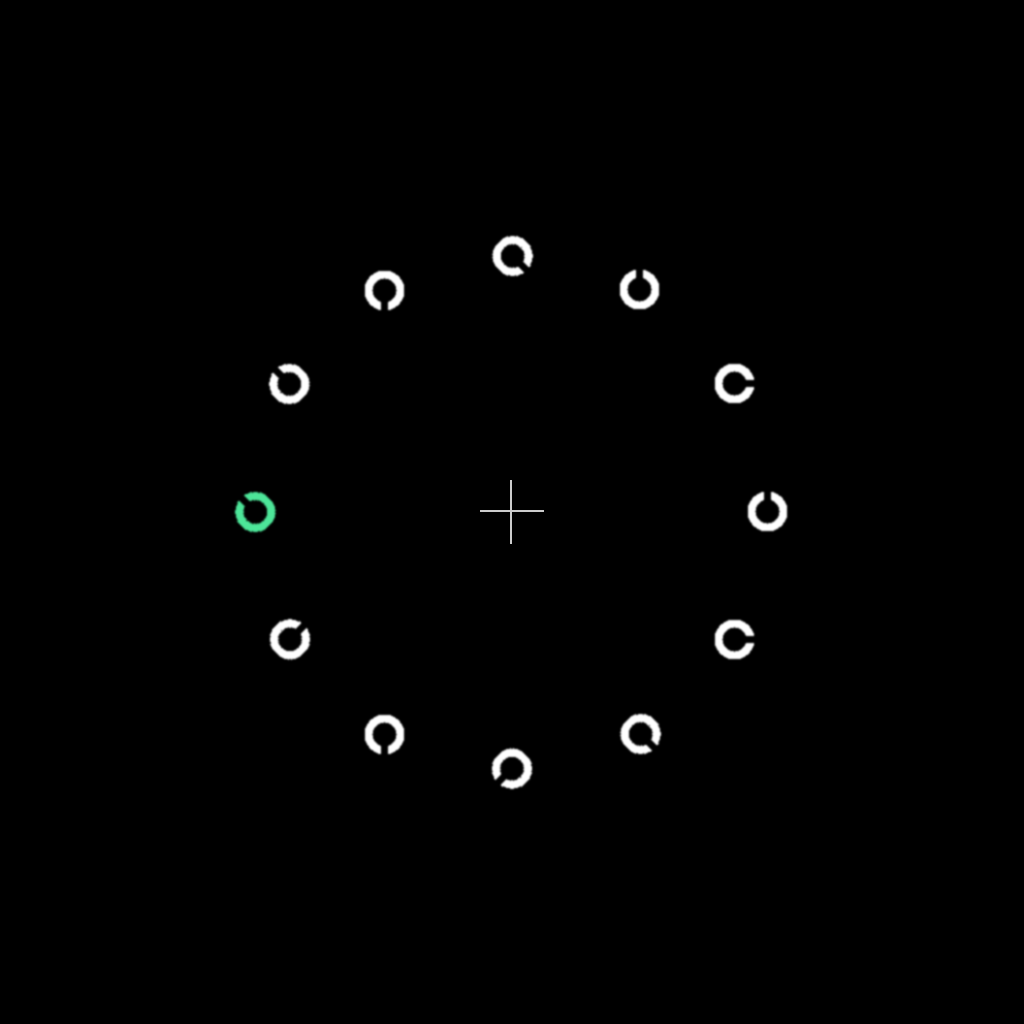
\includegraphics[width=6cm]{figs/exStimExp1.png}
\caption{Example stimulus from Experiment 1. Before the stimulus is shown, the observer is shown a green Landolt C. Their task is to decide if the green C in the stimulus matches.}
\label{fig:exp1stimulus}
\end{figure}

\subsubsection{Procedure}

\subsection{Results and Discussion}

blank


%%%%%%%%%%%%%%%%%%%%%%%%%%%%%%%%%%%%%%%%%%%%%%%%%%%%%
\section{Experiment 2}
\label{sec:exp2}
%%%%%%%%%%%%%%%%%%%%%%%%%%%%%%%%%%%%%%%%%%%%%%%%%%%%%

The aim of experiment two is to investigate whether the effect reported by \cite{reinhart2015} applies to more standard visual search paradigms, or if it is specific to the target matching task they used in their original study. Hence, in this study we remove the colour cue from the stimuli and change the observer's task from 'does the green item match the target template?' to 'is the taret present of absent in this stimulus?.' 

\subsection{Methods}

\subsubsection{Participants}

\subsubsection{Stimuli}

\subsubsection{Procedure}

\subsection{Results}

blank

\subsection{Discussion}

blank



%%%%%%%%%%%%%%%%%%%%%%%%%%%%%%%%%%%%%%%%%%%%%%%%%%%%%
\section{General Discussion}
\label{sec:discussion}
%%%%%%%%%%%%%%%%%%%%%%%%%%%%%%%%%%%%%%%%%%%%%%%%%%%%%


\begin{acknowledgements}
Thank you to Courtney Barr. 
\end{acknowledgements}

% BibTeX users please use one of
% \bibliographystyle{spbasic}      % basic style, author-year citations
%\bibliographystyle{spmpsci}      % mathematics and physical sciences
%\bibliographystyle{spphys}       % APS-like style for physics

\bibliographystyle{plainnat}
\bibliography{literature}

\end{document}
% end of file template.tex

